    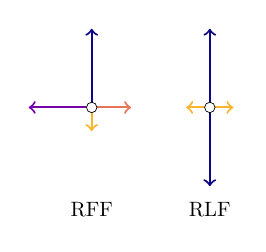
\begin{tikzpicture}\definecolor{color1}{RGB}{12,7,134}
\definecolor{color2}{RGB}{118,1,168}
\definecolor{color3}{RGB}{166,32,151}
\definecolor{color4}{RGB}{230,116,86}
\definecolor{color5}{RGB}{250,180,45}

        
        \draw[line width = 0.75, ->, color1] (0,0) -- (0,1);
        \draw[line width = 0.75, ->, color1] (0,0) -- (0,-1);
        \draw[line width = 0.75, ->, color5] (0,0) -- (0.3,0);
        \draw[line width = 0.75, ->, color5] (0,0) -- (-0.3,0);
        \node[draw, circle, scale =0.4, fill = white, line width = 0.25] at (0,0) {};
        
        
        
        \def\xspace{-1.5};

         \draw[line width = 0.75, ->, color1] (0+\xspace,0) -- (0+\xspace,1);
        \draw[line width = 0.75, ->, color5] (0+\xspace,0) -- (0+\xspace,-0.3);
        \draw[line width = 0.75, ->, color4] (0+\xspace,0) -- (0.5+\xspace,0);
        \draw[line width = 0.75, ->, color2] (0+\xspace,0) -- (-0.8+\xspace,0);

        \node[draw, circle, scale =0.4, fill = white, line width = 0.25] at (\xspace,0) {};
       
        \node[scale=0.75] at (0,-1.3) {\lstinline{RLF}};
        \node[scale=0.75] at (\xspace,-1.3) {\lstinline{RFF}};
        
        
    \end{tikzpicture}